\documentclass[10pt]{article}
\usepackage{natbib}
\usepackage[T1]{fontenc}
\usepackage[french]{babel}
\usepackage{xcolor}
\usepackage{url}
\usepackage[utf8x]{inputenc}
\usepackage{amsmath}
\usepackage{graphicx}
\usepackage{adjustbox}
\graphicspath{ {./images/} }
\usepackage{parskip}
\usepackage{fancyhdr}
\usepackage{vmargin}
\usepackage{cancel}
\usepackage{array}
\usepackage{caption}

\usepackage{dblfloatfix}


\setmarginsrb{1.1 cm}{1 cm}{1.1 cm}{1 cm}{0.75cm}{0.75 cm}{0.75 cm}{1.25 cm}


\title{Machine Learning Embarqué - Reconnaissance de styles}		% Title
\author{FIPA2022}								% Author
\date{\today}									% Date

\makeatletter
\let\thetitle\@title
\let\theauthor\@author
\let\thedate\@date
\makeatother

\pagestyle{fancy}
\fancyhf{}
\rhead{\theauthor}
\lhead{\thetitle}
\cfoot{\thepage}

\begin{document}

%%%%%%%%%%%%%%%%%%%%%%%%%%%%%%%%%%%%%%%%%%%%%%%%%%%%%%%%%%%%%%%%%%%%%%%%%%%%%%%%%%%%%%%%%

\begin{titlepage}
	\centering
    \vspace*{0.5 cm}
    
\includegraphics[scale = 0.75]{logo_ensta.png}\\[1.0 cm]	
    \textsc{\LARGE \newline\newline École d'ingénieur ENSTA Bretagne}\\[2.0 cm]	% University Name
	\textsc{\Large Machine Learning - FIPA 2022}\\[0.5 cm]				            % Course Code
	\rule{\linewidth}{0.2 mm} \\[0.4 cm]
	{ \huge \bfseries \thetitle}\\
	\rule{\linewidth}{0.2 mm} \\[1.5 cm]
	
	\begin{minipage}{0.5\textwidth}
        \begin{flushleft} \large
            \emph{Élève :} \\
			PETEREAU Elouan\\
			CAMICI Mathis\\
            \ \\
            \ \\
			
			\end{flushleft}
			\end{minipage}~
			\begin{minipage}{0.4\textwidth}
            
			\begin{flushright} \large
                \emph{Encadrants :}\\
                REYNET Olivier\\
                MORGE-ROLLET Louis\\
                \ \\
                \ \\
                
		\end{flushright}
        
	\end{minipage}\\[2 cm]
	
	
    \thedate
    
    
    
	
\end{titlepage}
\setlength\parindent{9pt}
%%%%%%%%%%%%%%%%%%%%%%%%%%%%%%%%%%%%%%%%%%%%%%%%%%%%%%%%%%%%%%%%%%%%%%%%%%%%%%%%%%%%%%%%%

\tableofcontents
\pagebreak

%%%%%%%%%%%%%%%%%%%%%%%%%%%%%%%%%%%%%%%%%%%%%%%%%%%%%%%%%%%%%%%%%%%%%%%%%%%%%%%%%%%%%%%%%


%%%%%%%%%%%%%%%%%%%%%%%%%%%%%%%%%%%%%%%%%%%%%%%%%%%%
% INTRODUCTION GENERALE                            %
%%%%%%%%%%%%%%%%%%%%%%%%%%%%%%%%%%%%%%%%%%%%%%%%%%%%
\section{Introduction générale}

Ce projet à pour objectif la comparaison des modéles de Machine Learning sur une plateforme embarqué. Pour cela, nous allons extraire les données depuis une database de musiques existantes, et déterminer le genre musical parmi ceux existant.

L'extraction de données se fera avec les algorithmes MFCC et STFT. Nous comparerons les modéles suivants:
Arbres de décision, Forêts d'arbres de décision, SVM, Réseaux de neurones

La plateforme utilisé sera une Raspberry Pi 4 en utilisant un OS Linux sur 64 bits. Nous devions utilisé les outils suivants: C++20, cmake(>=3.16), Python 3.9, Scikit Learn. Pur le training, nous avons choisi d'utiliser les versions suivantes : pandas (1.3.4), numpy (1.20.2), sklearn (1.0.1), matplotlib (3.4.0), graphviz (0.19.1). \\


\begin{figure}[h!]
\centering
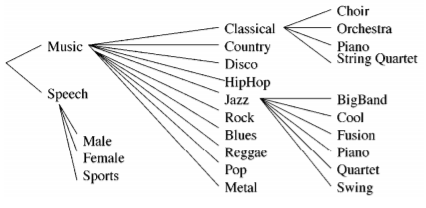
\includegraphics[width=0.4\textwidth]{listofgenre.png}
\caption{Listes des genres musicaux}
\end{figure}
Parmi l'ensembles des genres disponibles, nous avons choisis de retenir ceux présent dans la database que nous avons utilisé. Vous pouvez trouvez ci-dessous la liste des genres ainsi que l'organisation des fichiers du projet. 

\begin{minipage}[ht]{0.6\linewidth}
\centering
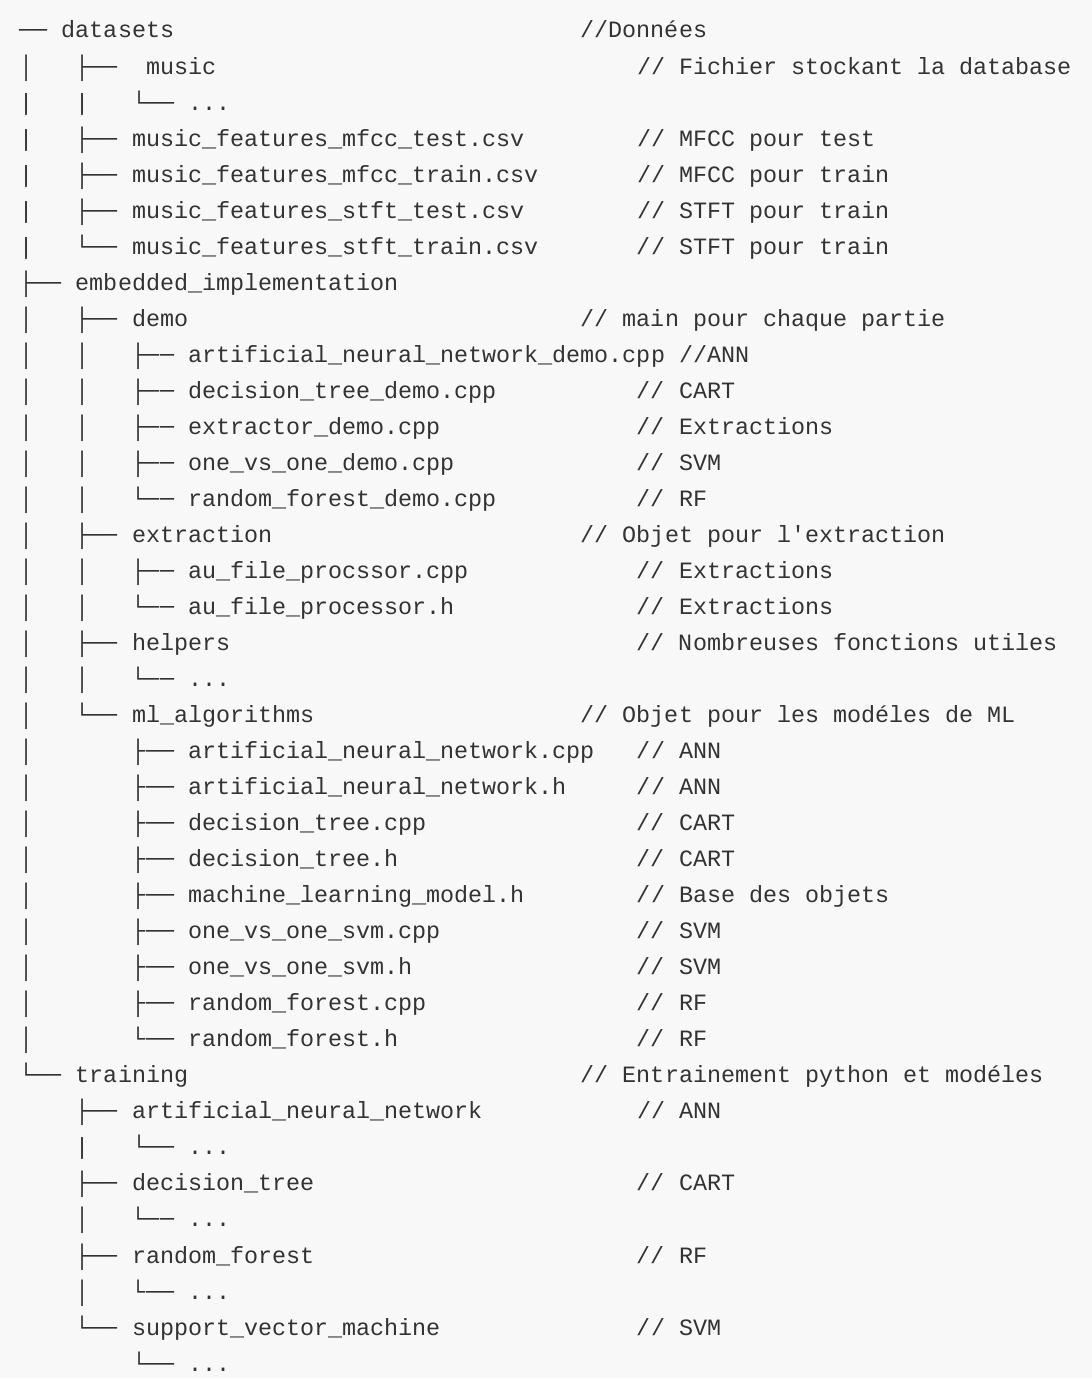
\includegraphics[width=0.9\textwidth]{DirectoryOrganisation.png}
\captionof{figure}{Organisation des fichiers du GitLab}
\end{minipage}
\begin{minipage}[h]{0.3\linewidth}
\begin{itemize}
  \item Classical
  \item Country
  \item Disco
  \item HipHop
  \item Jazz
  \item Rock
  \item Blues
  \item Reggae
  \item Pop
  \item Metal
\end{itemize}
\end{minipage}


%%%%%%%%%%%%%%%%%%%%%%%%%%%%%%%%%%%%%%%%%%%%%%%%%%%%
% EXTRACTION DES INFORMATIONS AUDIO                %
%%%%%%%%%%%%%%%%%%%%%%%%%%%%%%%%%%%%%%%%%%%%%%%%%%%%
\section{Extraction des informations audio}


\subsection{Lecture file extension .au}

\begin{minipage}[t]{0.4\linewidth}

\centering
\vspace{-2ex}
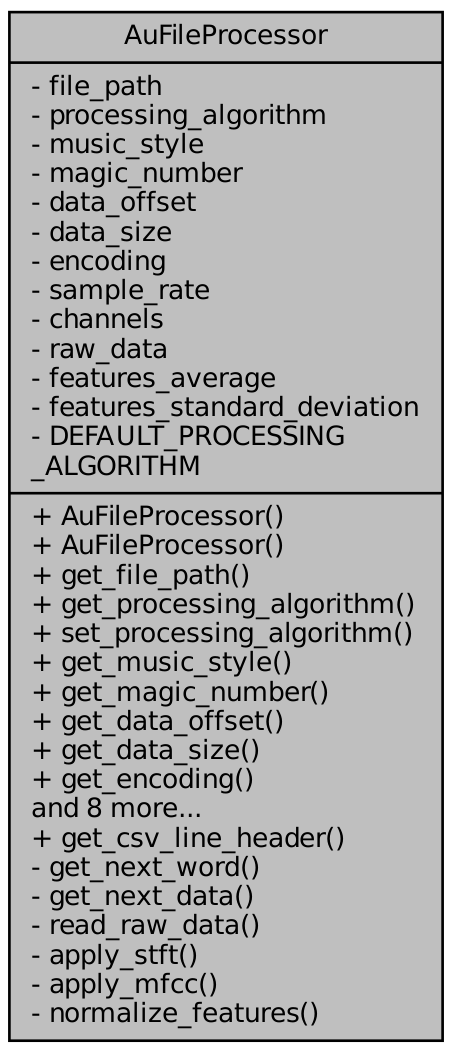
\includegraphics[width=0.55\textwidth]{UML-AuFIleProcess.png}
\captionof{figure}{UML Diagramme}

\end{minipage}
\begin{minipage}[t]{0.6\linewidth}
Nous débutons par l'extraction et la lecture de l'ensemble des fichier de la database GZTAN. Ces fichiers sont au format .au. La lecture de chaque fichier se fera à l'aide d'un objet, la classe AuFieProcessor. \\

Dans cette classe, nous retrouverons l'ensemble des informations du fichier comme le format, algorithme utilisé, le style de musique, le chemin...\\
Nous allons séparé les fichiers en deux catégories, pour l'apllication des algorithme de machine learning. Les deux parties sont TRAIN et TEST, commune à l'ensemble des algorithmes, on y retrouve respectivement 800 fichiers audio et 200 fichiers audio. \\

L'extraction se déroulera en plusieurs étapes. Tous d'abords, une partie en amont trie les fichiers selon les paramétres, elle trie avec TRAIN/TEST et STFT/MFCC. Ensuite, La fonction read\_file() permettera d'extraire les informations, puis, nous normalisons les données . Enfin, nous appliqueons soit la MFCC ou le STFT, dans process\_algorithm. Au final, les informations enregistrer seront la moyenne et l'écart type  obtenu à la fin des algorithmes. Ces informations seront disponible dans des fichiers csv global. \\ 

Le fonctionnement de read\_file() est le suivant : Au premier abords, nous allons récupérer les headers du fichiers. Nous vérifions que le magic number vaut 0x2e736e64, puis nous récupérons le data\_offset, le data\_size, enconding, sample\_rate, channels. Une fois les headers récupéres les donées pures que l'on stock dans raw\_data.
\end{minipage}%


\subsection{Extraction STFT}


Nous allons appliquer une Short-Time Fourier Transform. Nous allons travailler par windows, sur les raw\_data en sortie de read\_file(). Nous allons selectionner deux windows, de taille N, soit 512, que nous allons déplacé sur l'ensemble du signal. 

Sur ces windows, nous allons appliquer des Hamming Windows, puis une Fast Fourier Transform Iterative Direct. Afin d'obtenir la fréquence du signal. Ensuite, on effectuera la moyenne et l'écart type à la volée pour la valeur absolue de chaque fréquences, informations que l'on gardera et écrirera à un csv. Pour chaque musique, nous obtiendrons la moyenne et l'écart type de 256 fréquences.

Temps d'éxecution: $\approx 80$ Secondes.(Correspond au 1Go = 60 sec de traitements)\qquad Complexité: $ \mathcal{O}(TN log_2 N) \\ N: Number \hspace{0.2cm} of \hspace{0.2cm} samples \qquad T:Time \hspace{0.2cm} window $

\subsection{Extraction MFCC}

Nous allons appliquer une Mel Frequency Cesptral Coefficients. Cette algorithme débute tous comme la STFT. Avec le mêmes systémes de windows, suivi de Hamming Windows, et d'une FFT. 

Juste avant la FFT, nous retiendrons la log energy de chaque windows. Aprés la FFT, nous prendrons la valeur absolue de chaque fréquence. Sur ces valeurs absolues nous appliquerons un ensemble de filtres traingulaires, qui sont proportionnelle à la valeur de la fréquence. Nous ferons la somme pour obtenir une valeur par filtre. Ensuite, nous appliquerons une Discrete Consine Transform de type 2.\\
Nous pourrons calculer la moyenne et l'écart type pour chaqu'un des filtres, et de l'energie.

L'utilisation de la MFCC, est intéréssant car mêmes si son extraction est plus long, elle dimnune grandement la quantité d'informations (512 -> 42). Nous n'avons aucune perte d'informations, les algorithmes sont mêmes plus précis sur MFCC que sur STFT. En effet, les données MFCC reflétant mieux la sensibilité humaines

Temps d'éxecution: $\approx 95$ secondes \quad Complexité: $\approx \mathcal{O}(MTN log_2 N) \quad N: Number \hspace{0.2cm} of \hspace{0.2cm} samples \quad T:Time \hspace{0.2cm}window \hspace{0.3cm} M: Number of Filters$ 

Par la suite, nous essayerons les algorithmes sur les données STFT et MFCC. Nous conserverons le type de données donnant la meilleure précision.



%%%%%%%%%%%%%%%%%%%%%%%%%%%%%%%%%%%%%%%%%%%%%%%%%%%%
% Arbres de décision                               %
%%%%%%%%%%%%%%%%%%%%%%%%%%%%%%%%%%%%%%%%%%%%%%%%%%%%

\section{Arbres de décision}


\subsection{Generation automatique de csv pour executer la prise de décision sur cible}

Afin de construire l'algorithme du CART, nous avons choisi d'utiliser un Jupyter Notebook. Ce notebook nous permetera de créer le modéle, l'entrainer et aboutira à la création d'un fichier CSV avec l'ensemble des informations. Nous pourrons par la suite prendre les informations de ce fichiers pour executer la prise de décision sur cible.\\
Nous avons choisis de privilégiez la constitution d'un fichier de donnés plutôt que la génération automatique de code C++. En effet, cela nous permet d'avoir un arbre facilement modifiable en cas de changement et d'avoir des données moins lourdes pour construire le Random Forest.


Afin d'entrainer le modèle nous allons utiliser le modèle DecisionTreeClassifier de Sklearn. Grid Search et la cross validation nous permetteront d'obtenir le meilleur modèle possible. Nous allons faire varier la 'max\_depth' allant de 1 à 20. Nous allons au total faire 100 entrainements.

\subsection{Implementation du CART en paradigme objet}

\begin{minipage}[t]{0.4\linewidth}
\centering
\vspace{-2ex}
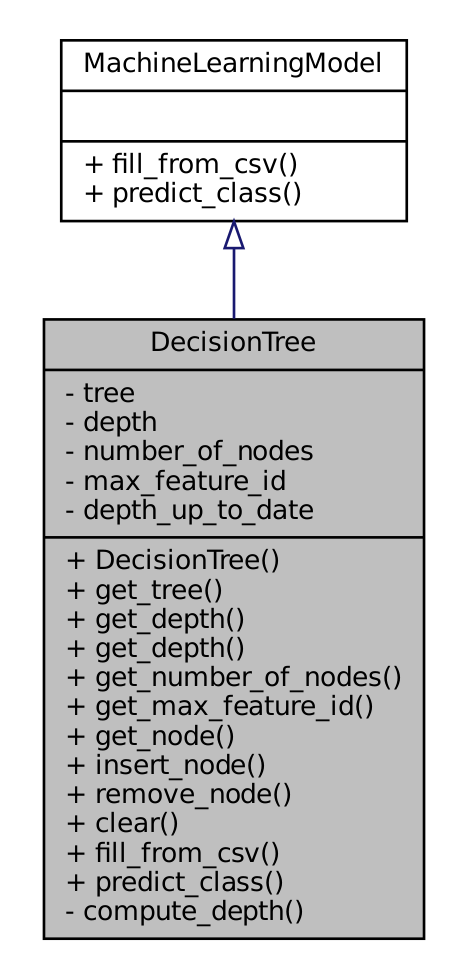
\includegraphics[width=0.6\textwidth]{DecisionTreeDiagram.png}
\captionof{figure}{UML Diagramme - Decision Tree}
\end{minipage}
\begin{minipage}[t]{0.6\linewidth}

Nous avons créé une classe appellé DecisionTree basé sur le modéle MachineLearningModel. Cette classe repose sur une autre classe TreeNode, qui correspond à chaque noeud de l'arbre et indiquant les conditions pour emprunter les branches suivantes. Notre arbre est donc composé de plusieurs TreeNode. \\

L'hors de l'éxécution sur cible, nous pouvons créer un arbre de décision fixe. pour cela nous pouvons ajouter des noeuds afin de constituer notre arbre, creant des instances de la classe TreeNode.\\

Un TreeNode est composé de son nom, d'un threshold, de son feature\_id (les données transformée issu de la partie extraction et du nom des ces enfants de droite et de gauche.\\

Les différentes fonction présente dans la classe sont des assesseurs des différentes caractéristiques de l'arbes. On peut ajouter et enlever des noeuds, supprimer entiérement l'arbre. On peut aussi obtenir la profondeur total de l'arbre. \\
La fonction fill\_from\_csv va lire un fichier csv et tant qu'il resetera de la données à lire. Elle lira chaque ligne, et pourra extraire l'id du node, le threshold, les données obtenu en extraction, les connections à gauche et à droite vers ses enfants, et son nom.\\


Complexité: $\approx \mathcal{O}(N)\quad N: \hspace{0.1cm} hauteur \hspace{0.2cm} de \hspace{0.2cm} l'arbre$ \\
Précision: STFT $\approx 0.44$ MFCC $\approx 0.49$\\
Les Matrices de confusion sont similaire sous Python et C++.
\end{minipage}

\begin{minipage}[t]{0.5\linewidth}

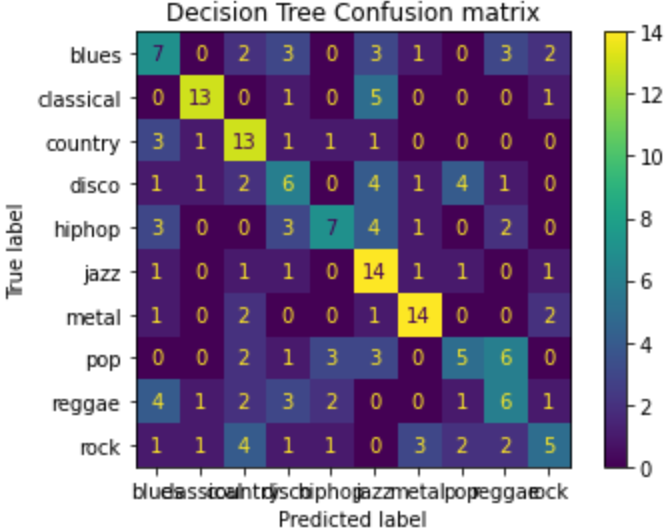
\includegraphics[width=0.7\textwidth]{DecisionTree-ConfusionMatrix.png}
\captionof{figure}{Matrice de Confusion - DecisionTree - STFT}

\end{minipage}
\begin{minipage}[t]{0.5\linewidth}

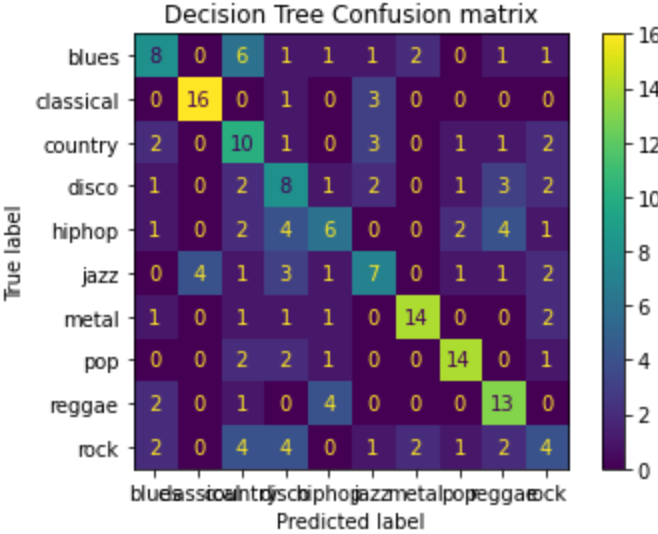
\includegraphics[width=0.7\textwidth]{DecisionTree-ConfusionMatrix2.png}
\captionof{figure}{Matrice de Confusion - DecisionTree - MFCC}

\end{minipage}

\subsection{Implementation du Random Forest basé sur le CART}

\begin{minipage}[t]{0.4\linewidth}
\centering
\vspace{-2ex}
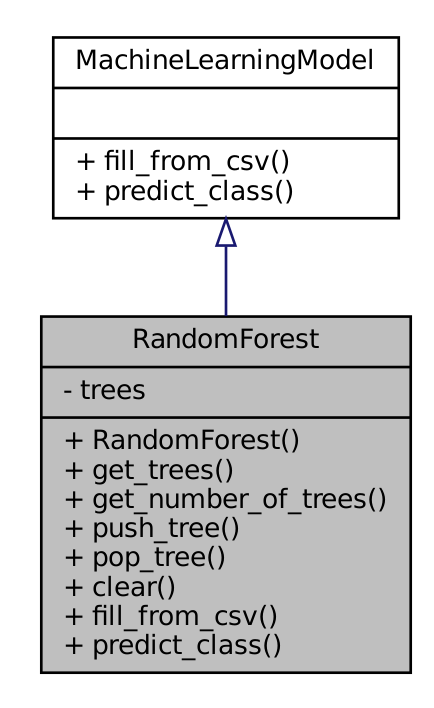
\includegraphics[width=0.8\textwidth]{RandomForestDiagram.png}
\captionof{figure}{UML Diagramme - Random Forest}

\end{minipage}
\begin{minipage}[t]{0.6\linewidth}
L'idée principale d'un RandomForest est d'avoir un certain nombre d'arbres de décision. Notre RandomForest se base sur des fichiers csv, ce sera un fichier par arbre.\\

Toutes les fonctions sont similaires à DecisionTree, vous pouvez ajouter des arbres, les supprimer ou effacer l'architecture.\\
La fonction predict\_class, calcule le résultat pour chaque arbre. Elle renvoie le résultat de la prédiction avec le plus de choix.\\
La fonction fill\_from\_csv, lit le répertoire, prend chaque fichier csv et crée un arbre de décision à partir de fill\_from\_csv déjà existant pour la classe DecisionTree et l'ajoute dans le RandomForest. \\

Pour entrainer le RandomForest, tous comme le DecisionTree, nous utilison un Jupyter Notebook. Nous allons utilisé RandomForestClassifier de Sklearn, avec GridSearchCV pour faire varier la profondeur de chaque arbre, le nombres d'arbres et le nombre d'échantillons à tirer  pour entraîner chaque estimateur.  \\

Complexité: $\approx \mathcal{O}(NM)\quad  N: \hspace{0.1cm} hauteur \hspace{0.1cm} de \hspace{0.1cm} l'arbre \hspace{0.2cm} M: \hspace{0.1cm} Nombre \hspace{0.1cm} d'arbre$ \\ 
Précision: STFT $\approx 0.57$ MFCC $\approx 0.60$ \\
Les Matrices de confusion sont similaire sous Python et C++.

\end{minipage}

\begin{minipage}[t]{0.5\linewidth}

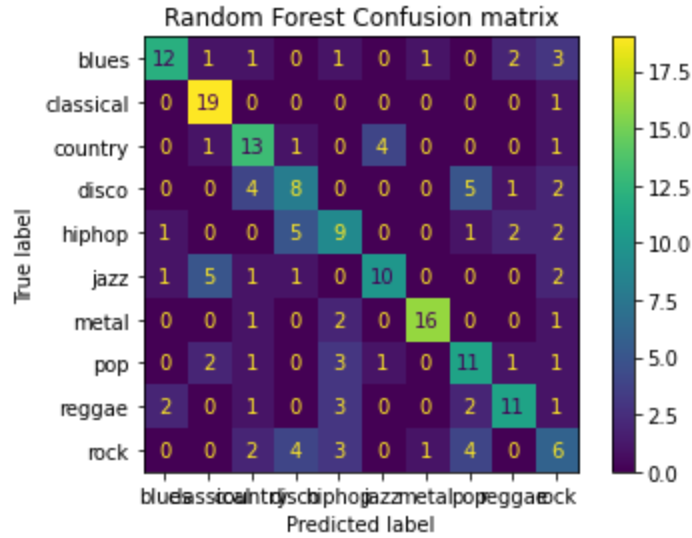
\includegraphics[width=0.7\textwidth]{RandomForest-ConfusionMatrix.png}
\captionof{figure}{Matrice de Confusion - RandomForest - STFT}

\end{minipage}
\begin{minipage}[t]{0.5\linewidth}

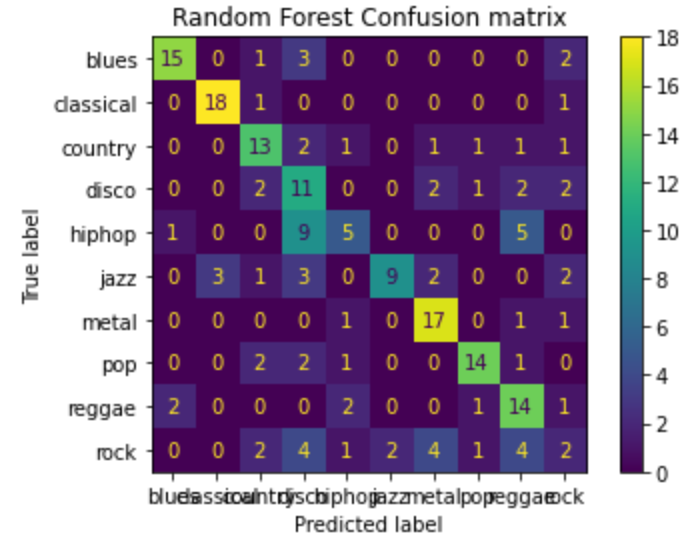
\includegraphics[width=0.7\textwidth]{RandomForest-ConfusionMatrix2.png}
\captionof{figure}{Matrice de Confusion - RandomForest - MFCC}

\end{minipage}
\vspace{0.2cm}



%%%%%%%%%%%%%%%%%%%%%%%%%%%%%%%%%%%%%%%%%%%%%%%%%%%%
% SVM                                              %
%%%%%%%%%%%%%%%%%%%%%%%%%%%%%%%%%%%%%%%%%%%%%%%%%%%%
\section{Séparateur à Vaste Marge}

\subsection{Elaborer une SVM optimale avec Scikit Learn}

Pour construire l'algorithme du SVM, nous avons choisis d'utiliser un Jupyter Notebook. Ce jupyter nous permetera de créer le modéle, l'entrainer, et aboutira à la création d'un fichier csv avec les différents coefficients et les différentes classes.

Afin d'entrainer le modéle, nous utilisons Sklearn et un GridSearchCV faisant varier C, un paramétre de régularisation. Il nous permet de faire varier la marge du modéle pour la ligne de décision, qui variera entre 0.1 et 20 avec un pas de 0.1. Nous avons aussi cherché à faire varier le kernel utilisé par l'alorithm entre lineaire, rbf (Gaussien), poly et sigmoid et optimisé chaque version selon les paramètres des kernels. La précision apporté par  rbf (Gaussien), poly et sigmoid était minime (moins de 0.5\%) mais nécessitait d'importants changements dans le code C++, nous avons donc choisis gardé un kernel linéaire.

\subsection{Implementation de la prediction un contre un sur cible}

Le SVM repose sur un principe de classification dépendant des frontiéres entre les données. En ajoutant une donnée nous pouvons voir dans quels frontiéres elle se situe, cela nous donne la prediction de sortie.

\begin{minipage}[t]{0.4\linewidth}
\centering
\vspace{-2ex}
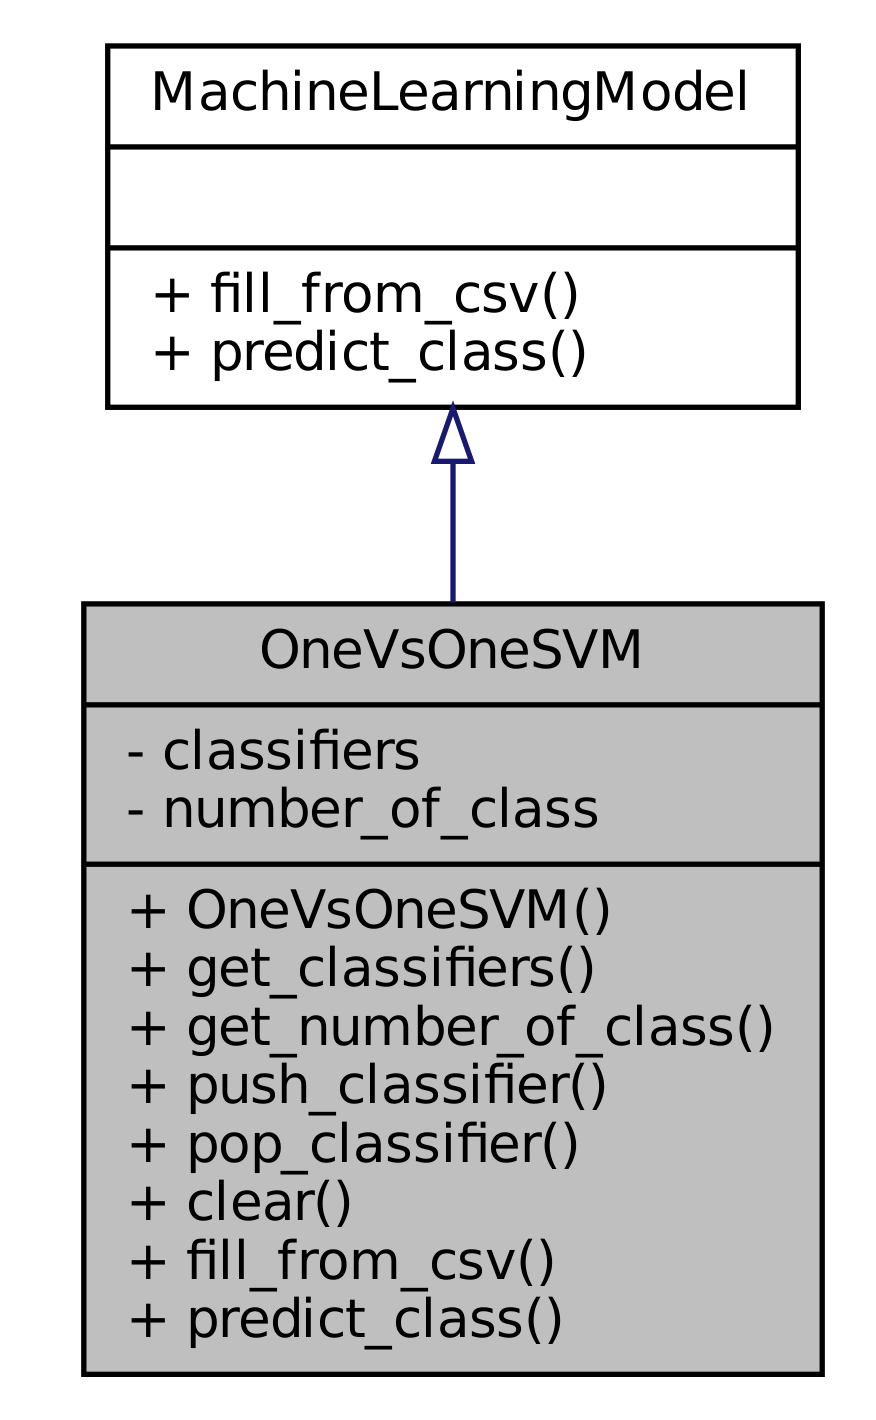
\includegraphics[width=0.8\textwidth]{SVMDiagram.png}
\captionof{figure}{UML Diagramme - Decision Tree}
\end{minipage}
\begin{minipage}[t]{0.6\linewidth}


L'algorithme OneVsOneSVM repose comme les anciens modéles sur un héritage de MachineLearningModel. Il est composé de plusieurs classifieurs présent dans la variable Classifiers, chaqu'un d'entre eux est basée sur un objet appellé LinearClassifier. \\
 
LinearClasifier est composé d'une classe négative et d'une classe positive, d'un Intercept et des coefficients de la matrice. Les classes négative et positive représentent les classes de décision confronté par le SVM e.g. pour la classe 1 contre 2 la classe positive sera 1 et basse 2. Cette objet met en place une fonction predict qui multiplie les coefficients du modéle avec les données de la partie extraction, puis fait la somme de ces résultats, additionne la valeur Intercept pour obtenir une seule valeur.Selon si le résultat est positif ou négatif nous renverrons la classe correspondante. \\


Pour les différents fonctions OneVsOneSVM:\\
Des accesseurs, nous permettant d'avoir accés au données suivante: la liste des LinearClassifiers, le nombre de classes.\\
push\_classifier, pop\_classifier, clear, nous permettant de gérer l'architecture. En effet, avec on peut ajouter un classifier, supprimer un ou l'ensemble des classifiers.\\
Fill\_from\_csv, permettant d'acceder au programe Python. Predict\_class, qui prends l'ensemble des résultats des différents LinearClassifier et renvoit le résultat ayant été sélectionneé le plus de fois. \\

Complexité: $\approx \mathcal{O}(N^{3}) \quad N:\quad Nombre \quad de \quad vecteurs \quad supports $ \\ 
Précision: STFT $\approx 0.66$ MFCC $\approx 0.71$\\
Les Matrices de confusion sont similaire sous Python et C++.
\end{minipage}
 
\begin{minipage}[t]{0.5\linewidth}

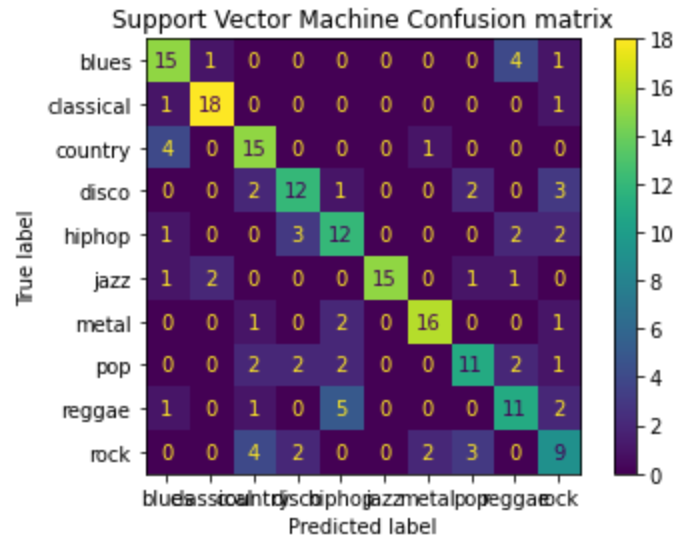
\includegraphics[width=0.7\textwidth]{SVM-ConfusionMatrix.png}
\captionof{figure}{Matrice de Confusion - SVM - STFT}

\end{minipage}
\begin{minipage}[t]{0.5\linewidth}

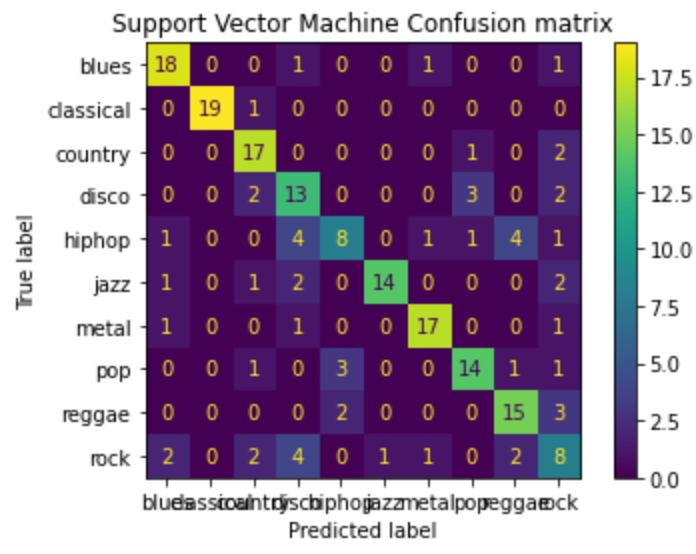
\includegraphics[width=0.7\textwidth]{SVM-ConfusionMatrix2.png}
\captionof{figure}{Matrice de Confusion - SVM - MFCC}

\end{minipage}
\vspace{0.2cm}


%%%%%%%%%%%%%%%%%%%%%%%%%%%%%%%%%%%%%%%%%%%%%%%%%%%%
% Réseau de neurones                               %
%%%%%%%%%%%%%%%%%%%%%%%%%%%%%%%%%%%%%%%%%%%%%%%%%%%%
\section{Réseau de neurones}


\subsection{Elaborer le modéle d'un réseau de neurones sur Python}

Le réseau de neurones décompose nos données en coches d'abstraction. Son comportement se définit par la façon dont ses éléments individuels sont reliées et par le poids sur chaque liaison. Ces poids s'ajustent au cours de l'entrainement. 

Nous avons ici utilisé Tensorflow pour créer le modéle. Il sera de 88 920 paramétres pour STFT et 1 494 paramétres pour MFCC. Nous avons choisis de construire une réseaux à deux couches d'avoir deux couches.\\
La premiére couche, ayant la mêmes taille que le nombre de données en entrées, avec une activation 'relu'. La seconde couche, ayant une taille de 10, pour les 10 genres possibles, et une activation 'softmax'.

La raison pour lesquelles nous avons choisis un réseaux simple était les difficultés d'entrainements. En effet malgrés de puissants GPU et des calculs d'une dizaine d'heures, nous n'avons pas pu trouver les bons paramétres pour le modéle. En d'autres termes, On peut constater que le modéle ne posséde pas les paramétres les plus optimiser, ce qui donne une précsion relativement faible.

\subsection{Implementation de la prédiction sur cible}

\begin{minipage}[t]{0.3\linewidth}
\centering
\vspace{-2ex}
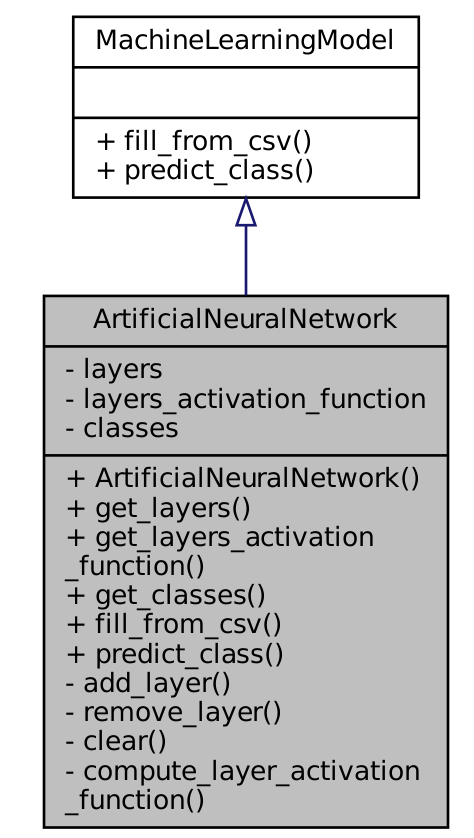
\includegraphics[width=0.85\textwidth]{ANNDiagram.png}
\captionof{figure}{UML Diagramme-ANN}
\end{minipage}
\begin{minipage}[t]{0.7\linewidth}
L'algorithme Artificial Neural Network reprends l'heritage de Machine Learning Model. Notre objet esr composé de plusieurs Neuron présent dans la variable layers.\\

Neuron, est un objet, il se compose d'une vecteur weights et d'un entier biais. Nous avons les accesseurs permettant d'accéder à ces deux variables. 
Puis, nous avons compute\_weighted\_sum, cette fonction multipliie les entrées avec chaque poids correspondant, puis additionne l'ensemble des valeurs obtenue, puis on additionne le biais. Cette valeur est ensuite renvoyer à l'ArtificialNeuralNetwork. \\

ArtificiaNeuralNetwork, a différentes variables et fonctions:\\
Parmi les variables, nous avons layers stockant l'ensemble des neurones, organiser en layers correspondant aux couches de neurones. \\
Puis layers\_activation\_function, stockant les fuctions d'activations nécessaires, les fonctions peuvent être SIGMOID, RELU, SOFTMAX. Dans notre cas, la premiére couche est RELU tandis que la deuxiéme est SOFTMAX.\\ Ensuite, classes indiquant pour la derniére couches, la correpsondance entre les neurones et les genres musicaux.\\

Parmie les fonction, nous avons  différents accesseurs pour accéder aux différentes variables. Ainsi que des fonctions nous permettant de gérer l'architecture de l'objet comme add\_layer, remove\_layer.\\
fill\_from\_cvs(), comme les anciens modéle, cette fonction vient chercher l'ensemble des données, et remplit les neurones avec les weights, les biaises et les classes.\\
predict\_class() est utilisé pour récuperer les valeurs des poids sommés, renvoyé par chaque neurones. Puis, va utiliser la fonction compute\_layer\_activation(). pour prendre soit une valeur positive du weight(RELU), soit prendre son exponentielle divisé par la somme des exponentielle de l'ensembe des weights. Une fois l'activation faite, nous prenons la valeurs max, et renvoyant la classe correspondante.\\


\end{minipage}



Complexité: $\approx \mathcal{O}(N) \quad N:\quad Nombre \quad de \quad Neurones  $ \\ 
Précision: STFT $\approx 0.70$ MFCC $\approx 0.64$ \\
Les Matrices de confusion sont similaire sous Python et C++.

\begin{minipage}[t]{0.5\linewidth}
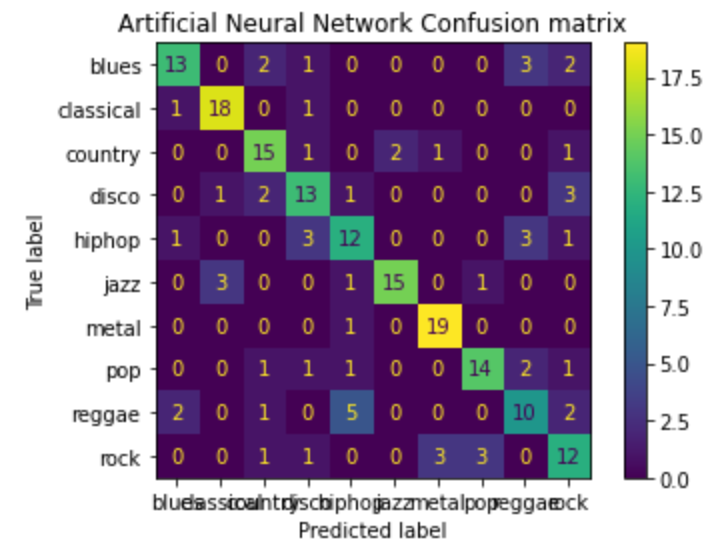
\includegraphics[width=0.7\textwidth]{ANN-ConfusionMatrix.png}
\captionof{figure}{Matrice de Confusion - ANN - STFT}

\end{minipage}
\begin{minipage}[t]{0.5\linewidth}

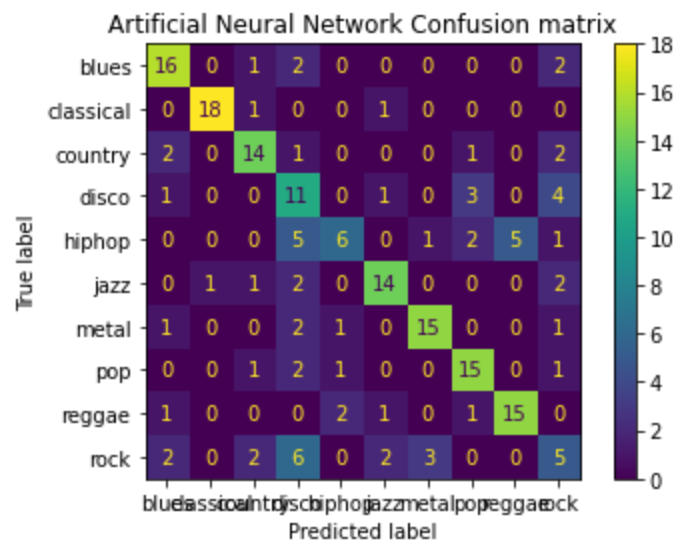
\includegraphics[width=0.7\textwidth]{ANN-ConfusionMatrix2.png}
\captionof{figure}{Matrice de Confusion - ANN - MFCC}

\end{minipage}

\pagebreak

%%%%%%%%%%%%%%%%%%%%%%%%%%%%%%%%%%%%%%%%%%%%%%%%%%%%
% Comparaison de l'ensemble des approches          %
%%%%%%%%%%%%%%%%%%%%%%%%%%%%%%%%%%%%%%%%%%%%%%%%%%%%
\section{Comparaison de l'ensemble des approches}

Nous avons pu implémenter l'ensemble des modéles sur la cible. Au vu de leurs fonctionnement respectives, nous avons pu comparer les approches et déterminer leurs caractéristiques respectives. \\ \\

 Tous d'abords, le CART était le modéle le plus rapide, le plus léger, cependant avec la précision la plus faible. Il apparait comme le meilleur modéle si nous avons peu de temps et peu de contraintes. 
 
 Ensuite, le RF, facile à implementer à partir d'un CART, apporte une forte complexité, une augmentation de taille importante. On note que la précision s'améliore relativement peu. Ce modéle peut être intéréssant si nous ne souhaitons pas embarquer la prédiction.

Puis, le SVM, le modéle qui nous parait le plus performant. Moins lourds et moins complexe que le RF. Il a la meilleur précision. Il est le meilleur modéle, dans notre cas, si nous avons suffisamment de temps pour l'implementer, et des contraintes de précison importantes.

Enfin, le ANN, le modéle le plus complexe. Ce modéle a la meilleur précision possible, sous reserve d'avoir une architecture bien choisis, et la puissance de calcul suffisantes pour l'optimiser. Dans notre cas, nous n'avons pas pu trouver une architecture optimiser malgré l'utilisation de puissant GPU et de calcul de plusieurs heures. \\ \\

De plus, nous avons pu voir que l'utilisation des données MFCC diminuait la compléxités des modéles, et mise à part le Réeau de Neurones, augmentait la précision.\\\\

Vous pouvez trouvez ci-joints des tableaux de caractérisitiques pour l'ensembles des modéles:\\

\begin{minipage}[t]{0.5\linewidth}

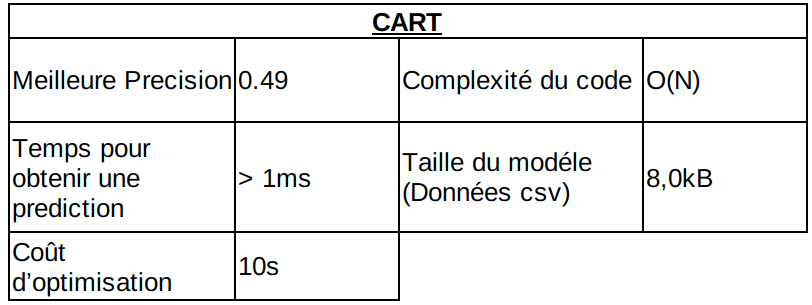
\includegraphics[width=\textwidth]{DecisionTree-FinalCompar.png}
\captionof{figure}{Tableau de Performances CART}

\end{minipage}
\begin{minipage}[t]{0.5\linewidth}

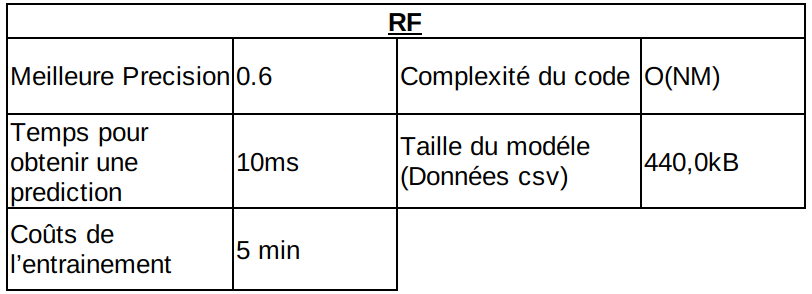
\includegraphics[width=\textwidth]{RF-FinalCompar.png}
\captionof{figure}{Tableau de Performances RF}

\end{minipage}
\newline
\newline
\newline
\begin{minipage}[t]{0.5\linewidth}

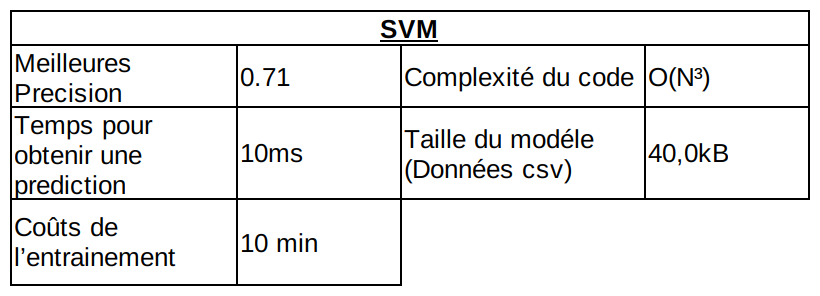
\includegraphics[width=\textwidth]{SVM-FinalCompar.png}
\captionof{figure}{Tableau de Performances SVM}

\end{minipage}
\begin{minipage}[t]{0.5\linewidth}

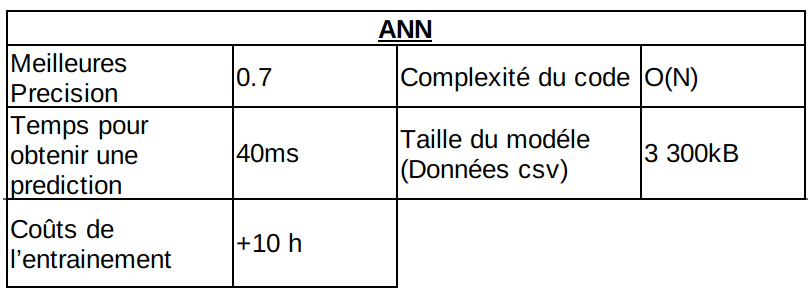
\includegraphics[width=\textwidth]{ANN-FinalCompar.png}
\captionof{figure}{Tableau de Performances ANN}

\end{minipage}



\end{document}